% Created 2026-02-25 Wed 15:41
% Intended LaTeX compiler: pdflatex
\documentclass[hidelinks, 11pt]{article}

\usepackage[utf8]{inputenc}
\usepackage[T1]{fontenc}
\usepackage{graphicx}
\usepackage{longtable}
\usepackage{wrapfig}
\usepackage{rotating}
\usepackage[normalem]{ulem}
\usepackage{amsmath}
\usepackage{amssymb}
\usepackage{capt-of}
\usepackage{hyperref}
\makeatletter \@ifpackageloaded{geometry}{\geometry{margin=2cm}}{\usepackage[margin=2cm]{geometry}} \makeatother
\usepackage{siunitx}
\usepackage{amsmath}
\usepackage{amssymb}
\usepackage{mathtools}
\usepackage{circuitikz}
\usepackage{float}
\usepackage{karnaugh-map}
\usepackage[sfdefault]{plex-sans}
\usepackage[scale=0.90]{plex-mono}
\usepackage{fancyhdr}
\pagestyle{fancyplain}
\lhead{Bach \textsc{Wongwandanee}}
\rhead{ECE 403}
\chead{Assignment 6}
\author{Waridh (Bach) Wongwandanee}
\date{\today}
\title{ECE 403 Assignment 6}
\hypersetup{
 pdfauthor={Waridh (Bach) Wongwandanee},
 pdftitle={},
 pdfkeywords={},
 pdfsubject={},
 pdfcreator={},
 pdflang={English}}
\usepackage{biblatex}

\begin{document}

\section*{Question 1}
\label{sec:org2bca8aa}
Non-idealities that increase the MOSFET \(I_{DS}\) when on vs the Shockley model.

The Shockley model is available in (\ref{eq-shockley}).

\begin{equation}
\label{eq-shockley}
  I_{DS} = \begin{cases}
    0 & \text{if cutoff} \\
    \beta\left( \left( V_{GS} - V_{TH} \right) V_{DS} - \frac{V_{DS}^2}{2} \right) & \text{if linear} \\
    \frac{\beta}{2} \left( V_{GS} - V_{TH} \right)^2 & \text{if saturation}
  \end{cases}
\end{equation}

\begin{equation}
\label{eq-channel-length-modulation}
I_{DS} = \frac{\beta}{2} \left( V_{GS} - V_{TH} \right)^2 \left( 1 + \lambda V_{DS} \right)
\end{equation}

\begin{equation}
\label{eq-body-effect}
V_t = V_{t0} + \gamma \left( \sqrt{\phi_s + V_{sb}} - \sqrt{\phi_s} \right)
\end{equation}

\begin{equation}
\label{eq-subthreshold-leakage}
I_{DS} = I_{DS0} \exp \left( \frac{V_{GS} - V_{t0} + \eta V_{DS} - k_\gamma V_{sb}}{n v_T} \right) \left( 1 - \exp \left( \frac{-V_{DS}}{v_T} \right) \right)
\end{equation}

\begin{description}
\item[{Channel length modulation}] Seen in (\ref{eq-channel-length-modulation}), channel length modulation increases \(I_{DS}\) over the Shockley model.
\item[{Decreasing \(V_{TH}\)}] The different effects that decrease \(V_{TH}\) will increase \(V_{GS} - V_{TH}\) which in turns increases the value of \(I_{DS}\).
There are some effects that decreases \(V_{TH}\)
\begin{description}
\item[{Body effect}] By decreasing \(V_{sb}\), especially below 0, (\ref{eq-body-effect}) shall decrease \(V_{TH}\), which then increases \(I_{DS}\).
\item[{Short Channel effect}] By decreasing the channel length, \(V_{TH}\).
\end{description}
\item[{Subthreshold leakage}] Technically, since the expected Shockley model at cutoff is \qty{0}{A}, then having a non-zero value is more. The subthreshold leakage is available in (\ref{eq-subthreshold-leakage}).
\end{description}
\section*{Question 2}
\label{sec:org29f45bb}
The dual rail domino XOR-3 gate requires the complement function of a XOR-3.
We are going to first define the definition for the regular XOR-3.
The XOR-3 function outputs 1 when an odd number of inputs are 1, and 0 otherwise.
The negation of the XOR-3 would be a XNOR-3, which outputs 1 when there is an even number of 1 in the input. This is described in (\ref{eq-xor}), and (\ref{eq-xnor}).

\begin{equation}
\label{eq-xor}
\text{XOR-3} = A \overline{B} \overline{C} + \overline{A} B \overline{C} + \overline{A} \overline{B} C + A C B
\end{equation}

\begin{equation}
\label{eq-xnor}
\text{XNOR-3} = \overline{A} B C + A \overline{B} C + A B \overline{C} + \overline{A} \overline{B} \overline{C}
\end{equation}

After finding these equations, the XOR-3 gate using dual rail domino logic is available in figure \ref{fig-opt-xor}.

\begin{figure}[htbp]
\centering
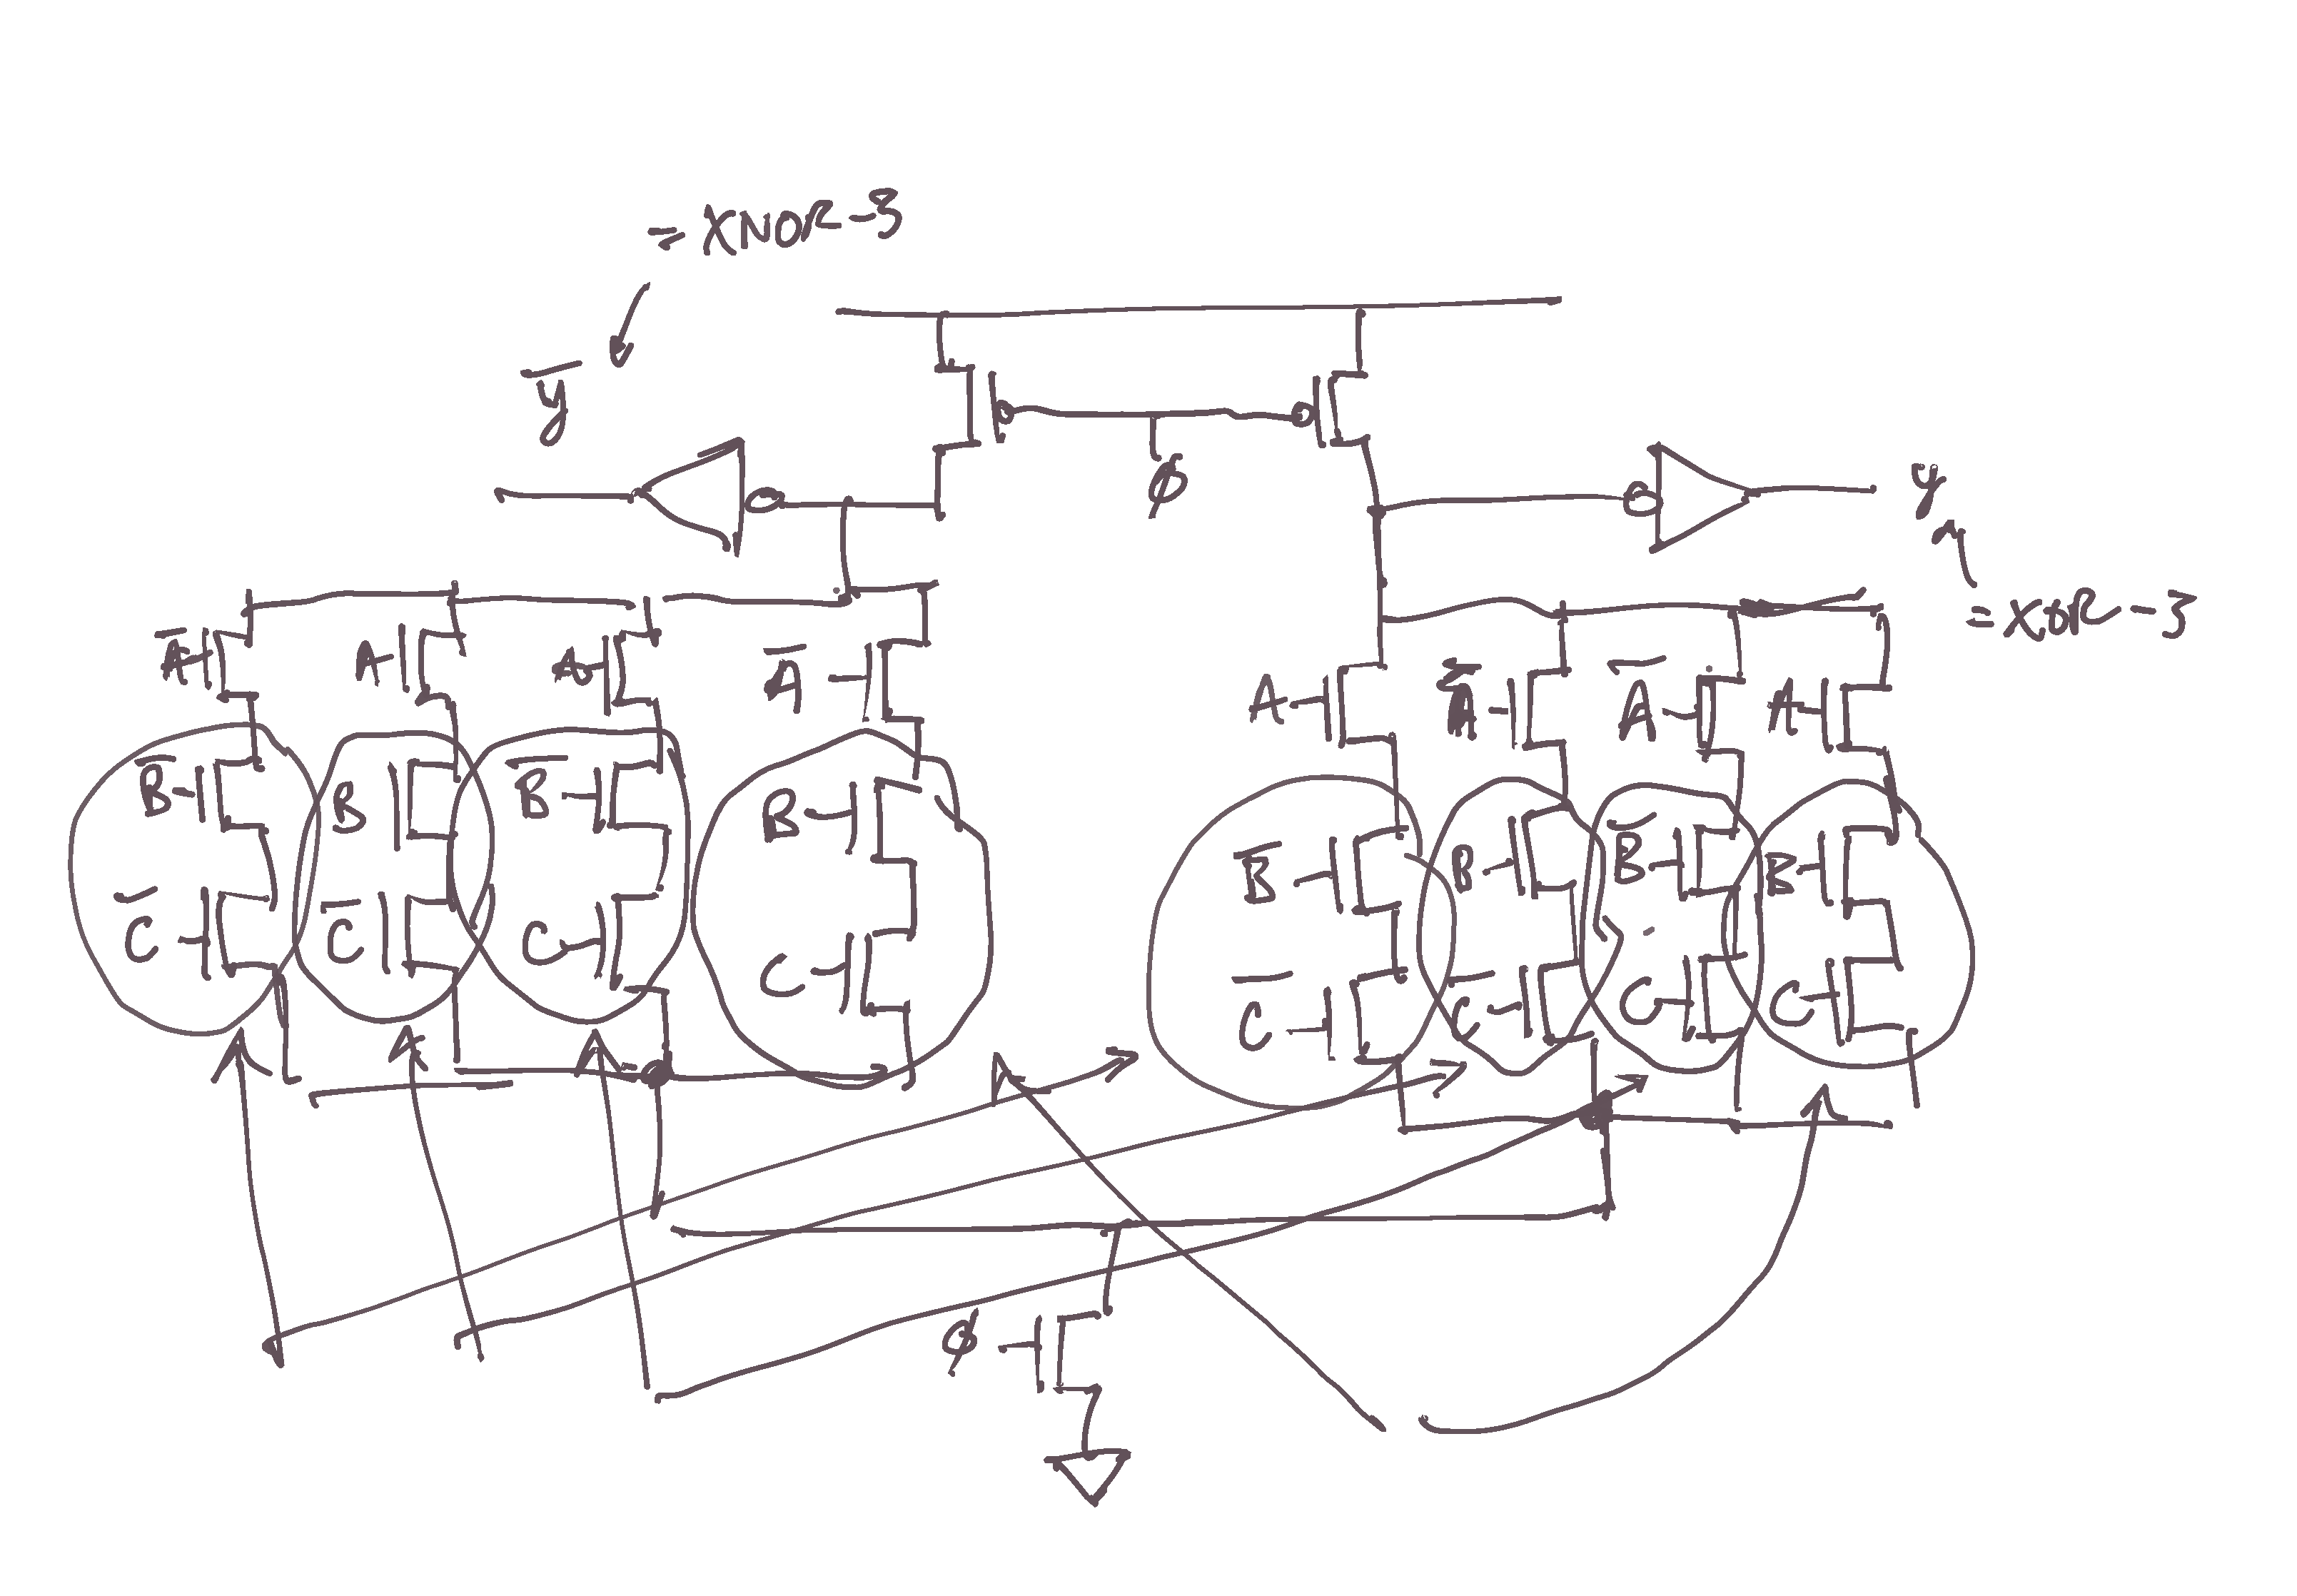
\includegraphics[width=0.7\linewidth]{images/unopt.pdf}
\caption{\label{fig-unopt-xor}The unoptimized XOR-3 gate.}
\end{figure}

\begin{figure}[htbp]
\centering
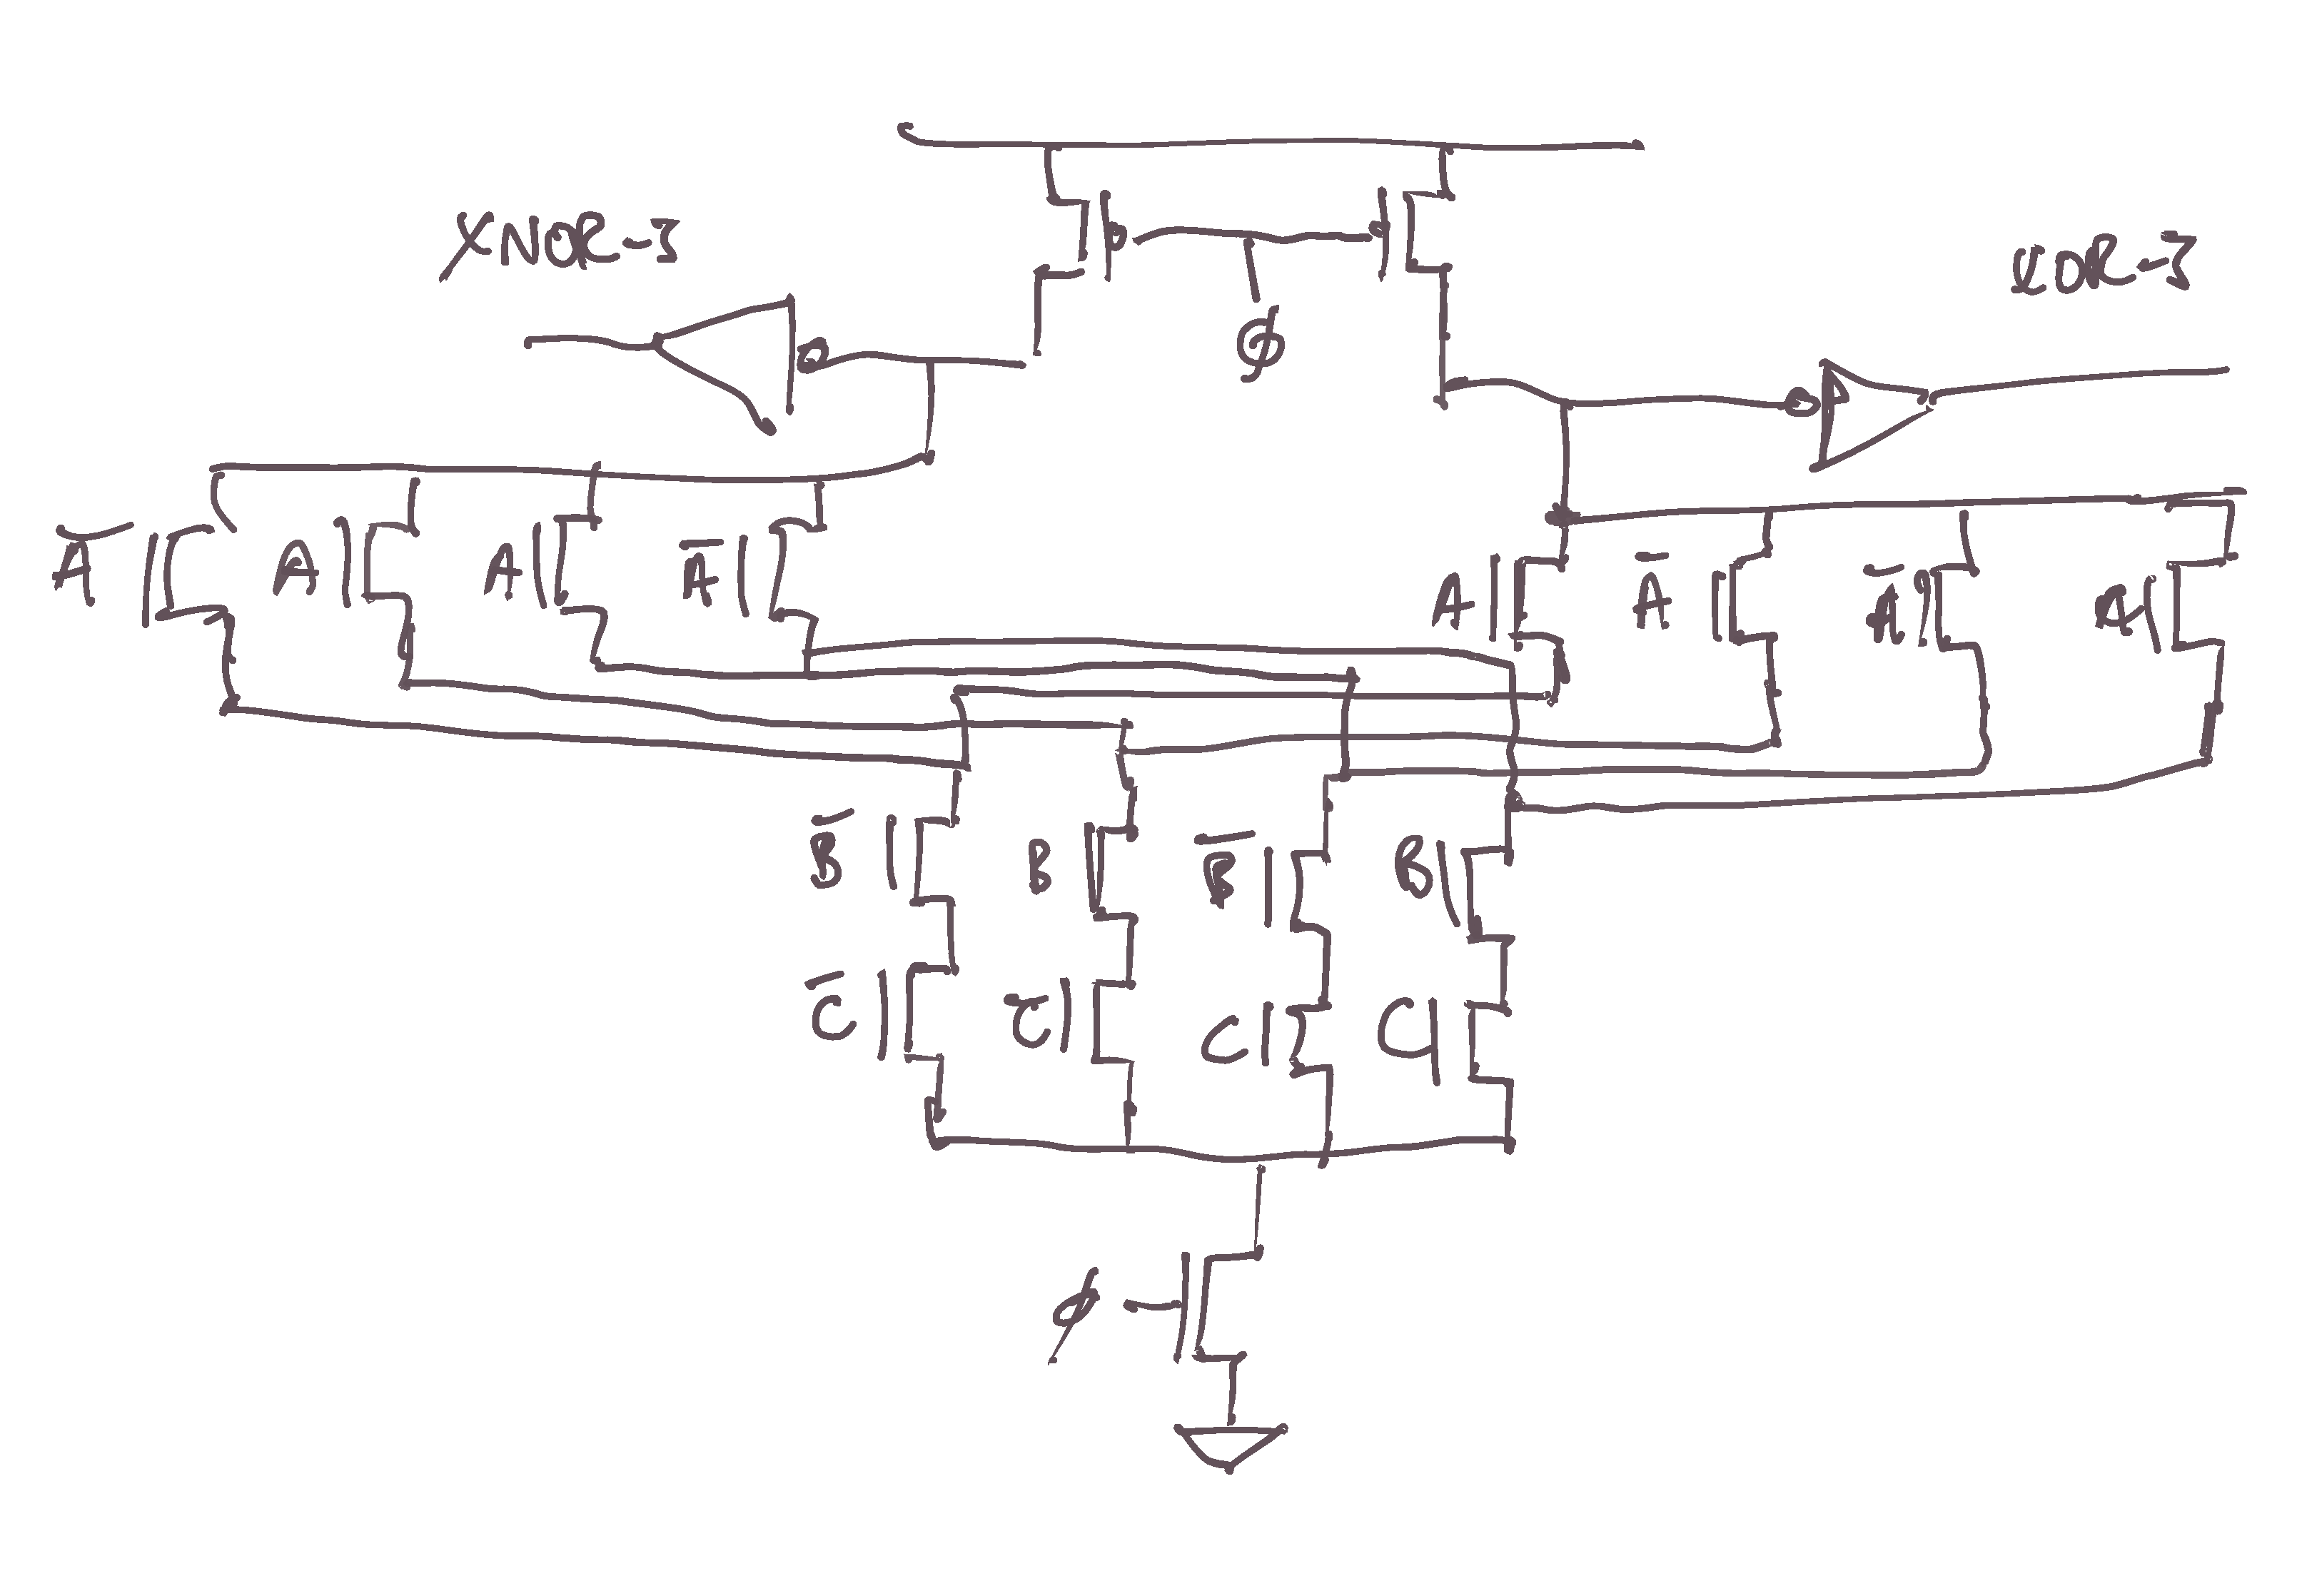
\includegraphics[width=0.7\linewidth]{images/little-opt.pdf}
\caption{\label{fig-little-opt-xor}Intermediate XOR-3 gate.}
\end{figure}

\begin{figure}[htbp]
\centering
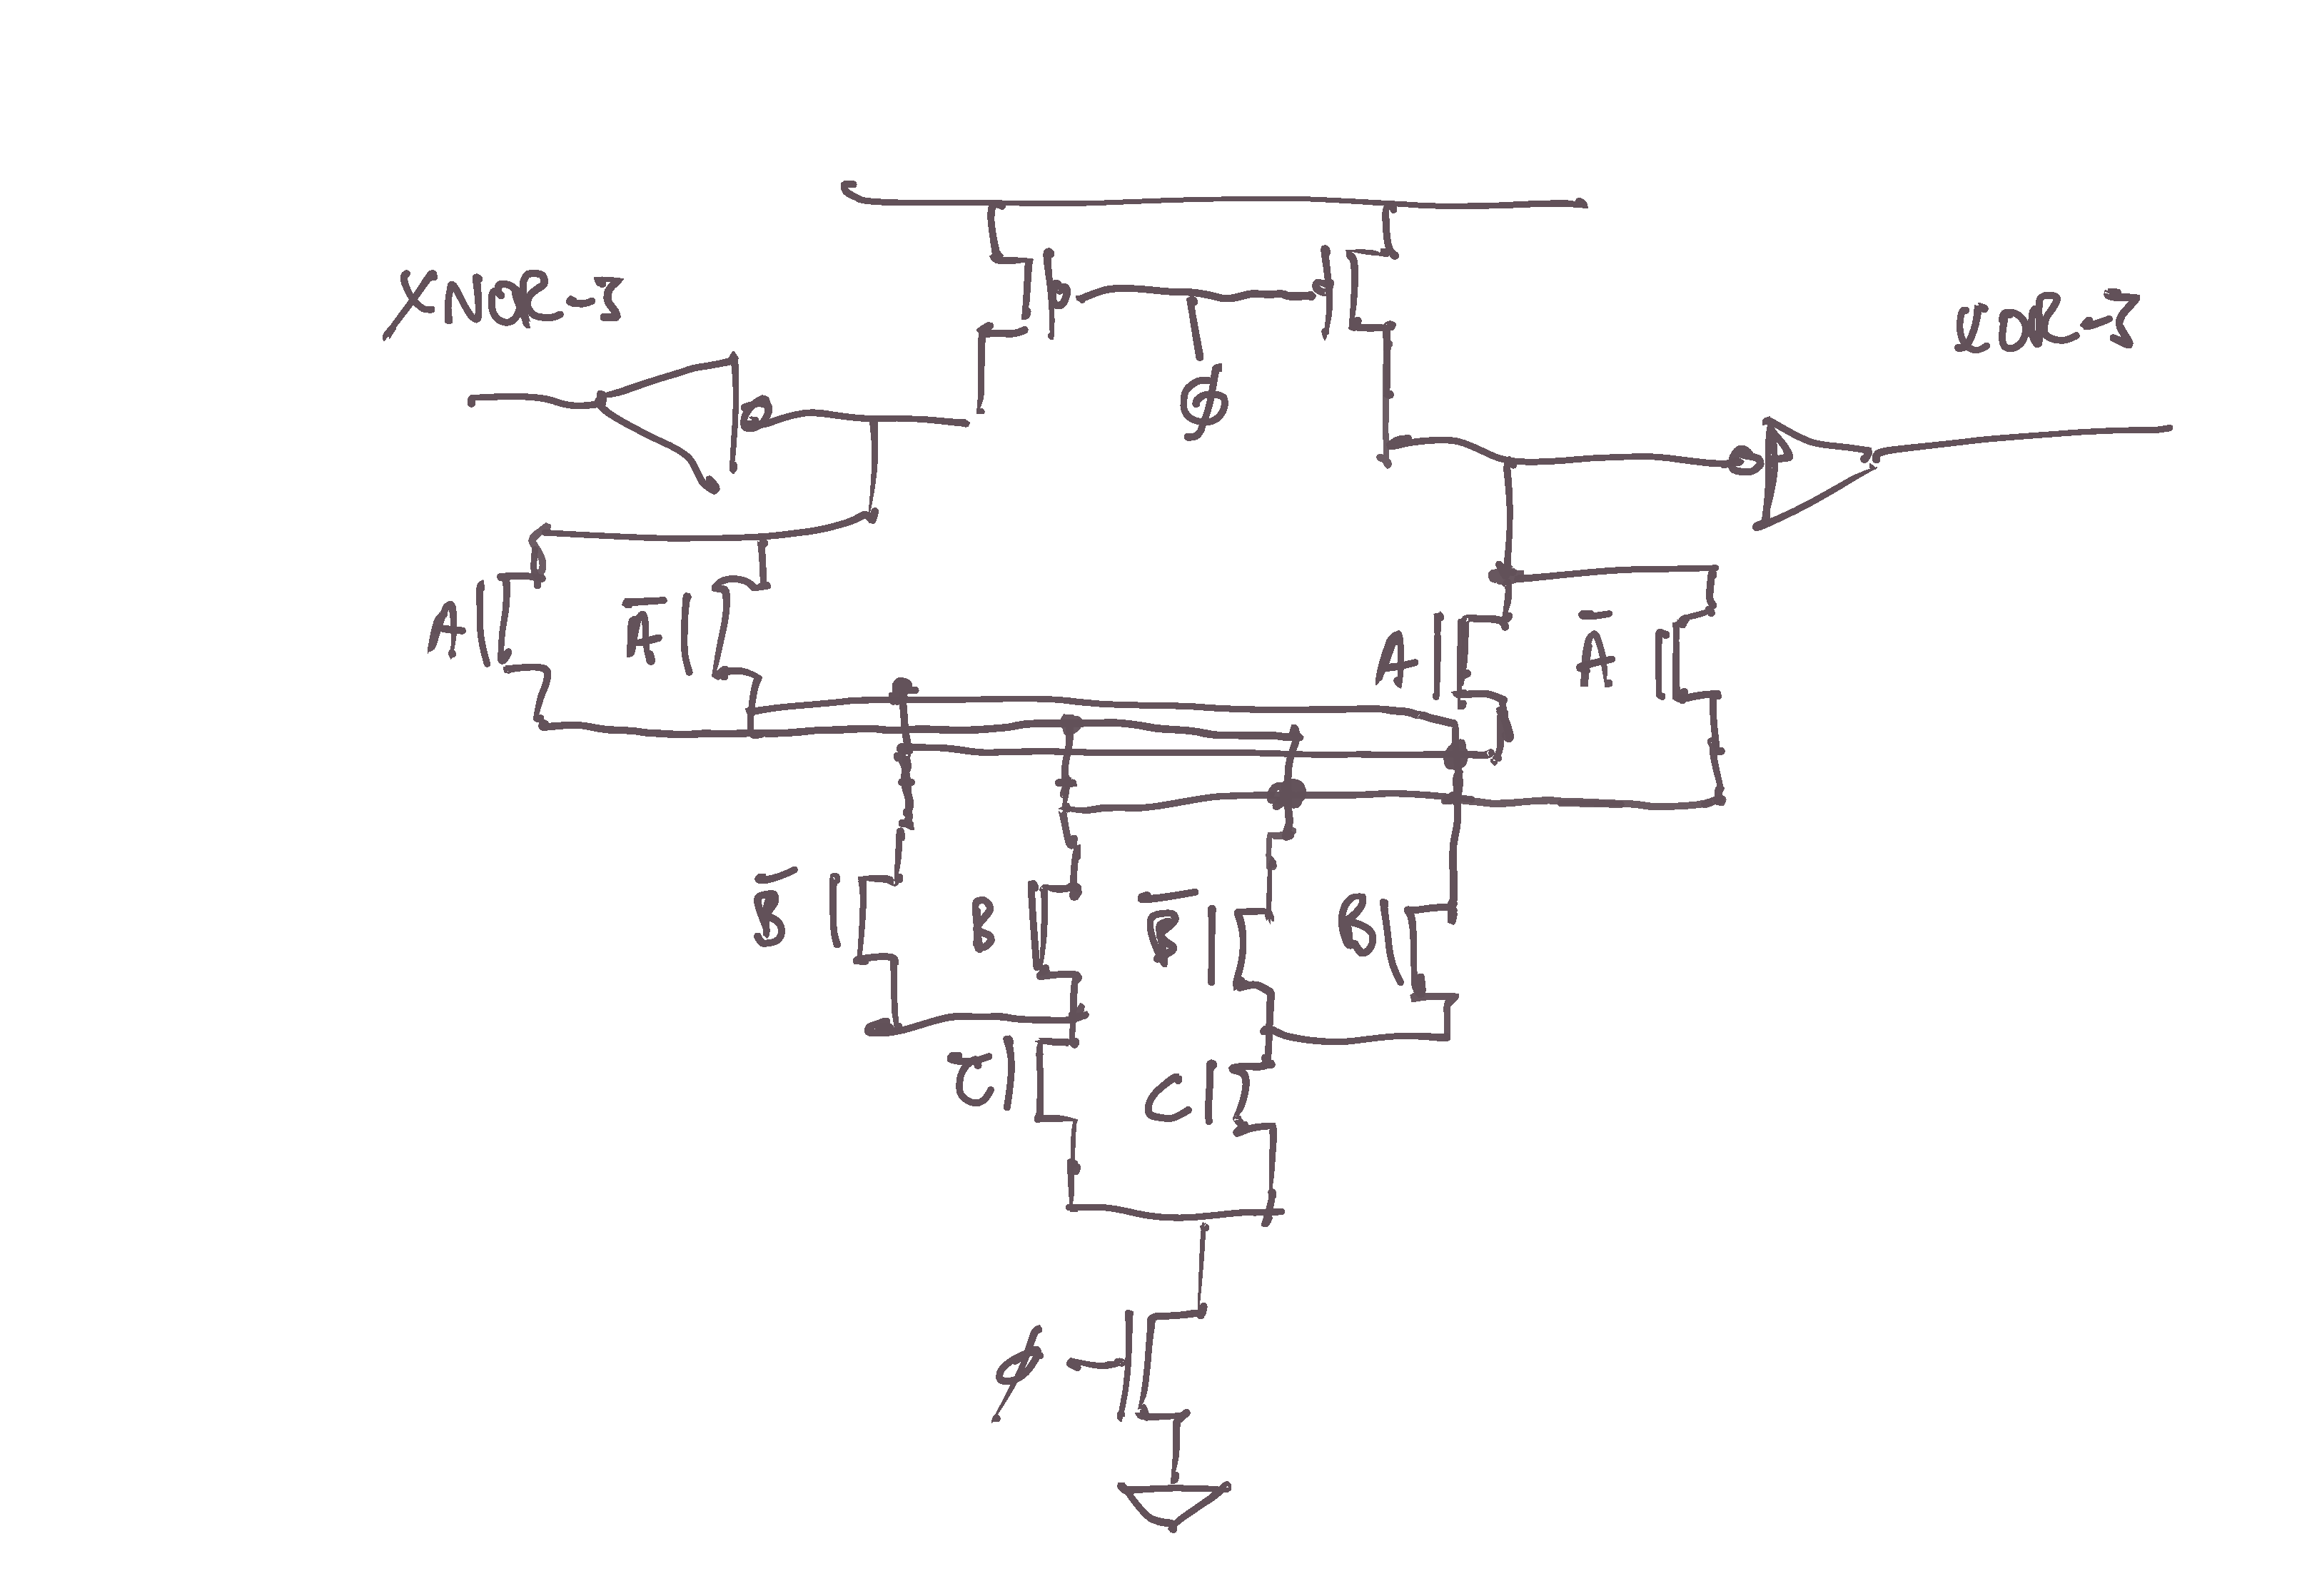
\includegraphics[width=0.7\linewidth]{images/opt.pdf}
\caption{\label{fig-opt-xor}Optimized XOR-3 gate.}
\end{figure}
\end{document}
